%! TeX root = report.tex

\section{M1: Spec 1}

\begin{figure}
    \centering
    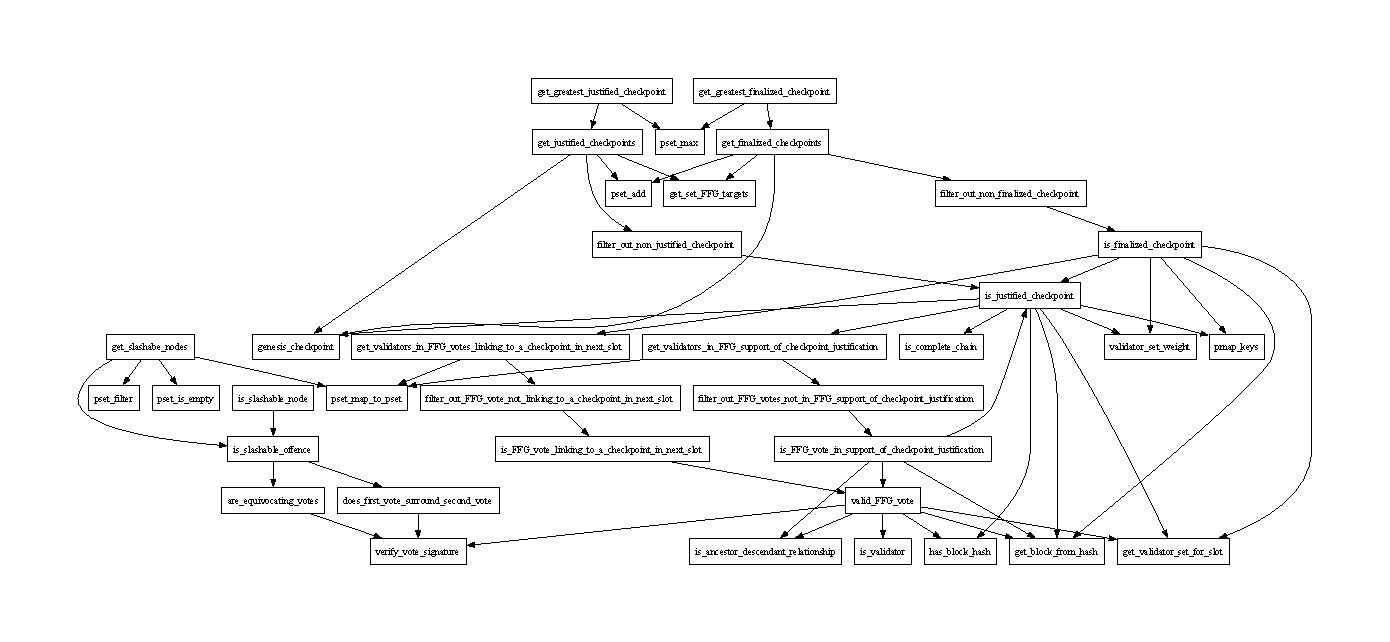
\includegraphics[width=\textwidth,angle=-90]{ffg-callgraph.pdf}
    \caption{The callgraph of the 3SF specification}
    \label{fig:your_label}
\end{figure}

The first specification is obtained by following the principle of least surprise; to the extent that it is possible, without regard to model checking efficiency, we translate Python code to its \tlap{} counterpart with the closest syntax, preserving semantics.

Despite being a programming language and specification language respectively, Python and \tlap{} overlap somewhat in what they can express. 
For instance, both allow us to express sets, and then filter those sets by a given predicate to obtain a different set.
To take a concrete example, observe the definition of \textsf{pset\_filter} in Figure~\ref{py_filter}.
\begin{figure}
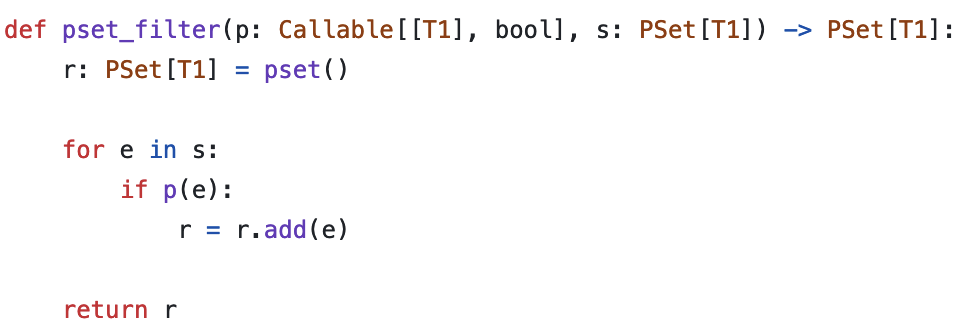
\includegraphics[width=\textwidth]{images/pset_filter.png}
\caption{\textsf{pset\_filter} definition \label{py_filter}}
\end{figure}
%
Notice that, while filter is not one of the built-in operators of the \emph{pyrsistent} library, it is relatively simple to define a filter operator, such that the set returns contains exactly all of the elements of $s$, for which the Boolean predicate $p$ holds true.
In \tlap{}, however, filtering is a language primitive, so if we can translate a python set $s$ to a \tlap{} set $\hat{s}$, and a Python predicate $p$ (of the above type) to a \tlap{} predicate $\hat{p}$, we can translate $\mathsf{pset\_filter}(p, s)$ to $\{ x \in \hat{s}\colon \hat{p}(x) \}$.

We take this idea, and apply it to every definition in the file \texttt{pythonic\_code\_generic.py}, attempting to identify \tlap{}-equivalents (w.r.t. semantics) for each defined function. 
Later on, in Section~\ref{section3}, we give a formal characterization of all of these equivalencies, in the form of rewriting rules, although for the purposes of this first specification, the entirety of this translation is manual.

Although it is relevant in the process of translation, we do not give explicit rules for the translation of Python language primitives to \tlap{} in general, since attempting to establish those for the full language would vastly exceed the scope of this project. 
Some of these constructs are particularly relevant, and we briefly mention them here:
\paragraph{Assignments and local variables.} There are certain idiosyncrasies to do with the fact that one language is executable, and the other is not. For instance, Python allows for arbitrary variable assignment and reassignment, as well as the introduction of local variables. There are two constructs available in \tlap{} which can be used to express variable assignment:
\begin{itemize}
  \item state-variable update $a' = e$
  \item LET-IN local operator definition $\mathrm{LET}\; v \defeq e \;\mathrm{IN}\; f$
\end{itemize}
to avoid going in to too much detail, it is up to the translator to evaluate which of the two better captures the semantics of the Python code (with, in general, a preference for the LET-IN variant).
\paragraph{Runtime exceptions.} Python code may throw at any time, sometimes in the form of Require-assertions within function definitions. 
In general, this behavior is impossible to replicate without very convoluted \tlap{} code, so we either have to omit those assertions, or return an unspecified value of the correct type if the requirement is not met.

\paragraph{Recursion.} Native \tlap{} supports recursive operators at the language level, but Apalache does not, at the model-checking level. This means that we can translate recursive Python functions as-written in \texttt{Spec 1}, with the knowledge that we will need to remove them in \texttt{Spec 2} to facilitate model checking.

As an example, Figure~\ref{py_adr} shows a crucial operator, \textsf{is\_ancestor\_descendant\_relationship}, as it is expressed in Python, and Figure~\ref{tla_adr} shows its \tlap{} equivalent.
\begin{figure}
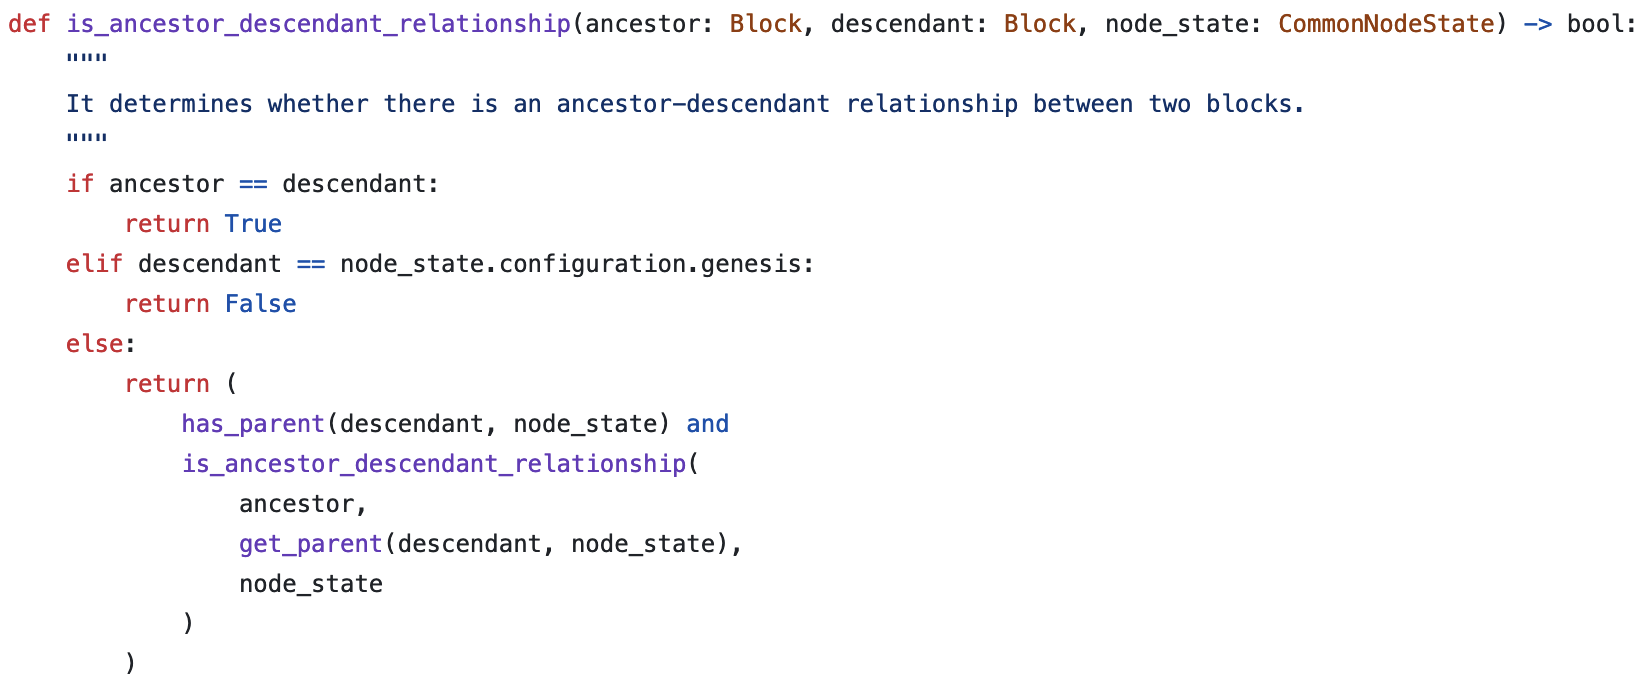
\includegraphics[width=\textwidth]{images/is_ancestor_descendant_relationship.png}
\caption{\textsf{is\_ancestor\_descendant\_relationship} Python definition \label{py_adr}}
\end{figure}

\begin{figure}
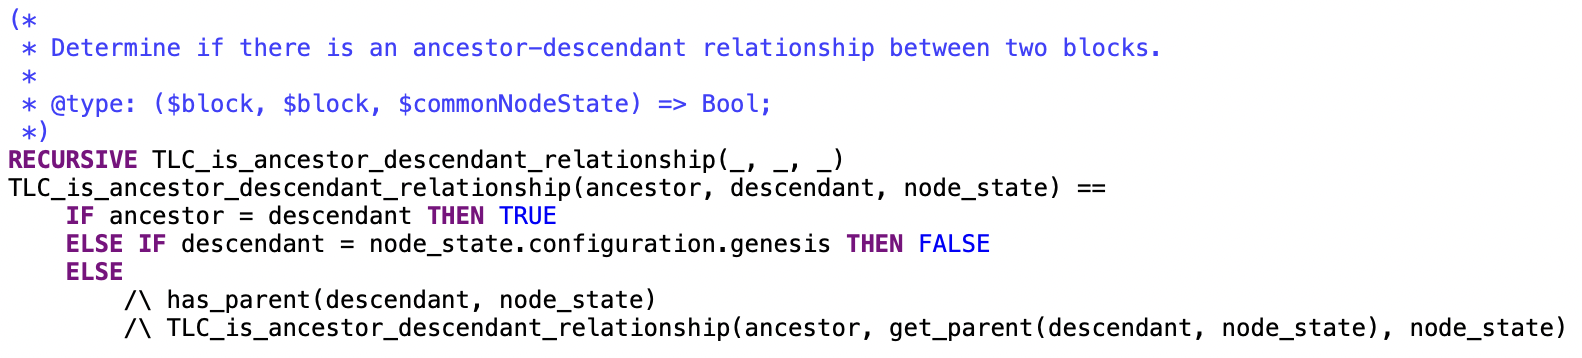
\includegraphics[width=\textwidth]{images/TLC_is_ancestor_descendant_relationship.png}
\caption{\textsf{is\_ancestor\_descendant\_relationship} \tlap{} equivalent \label{tla_adr}}
\end{figure}
%
We can see that the \tlap{} specification requires us to explicitly annotate the operator as recursive. 
Beyond that, since both languages support if-statements, those translate directly (though since \textsf{elif} in Python has no equivalent, we chain two ifs). 
Lastly, the \tlap{} operator references \textsf{has\_parent} and \textsf{get\_parent}, which are \tlap{}-translated python operators themselves. 
In summary, this example demonstrates that our translation strongly preserves the syntactic shape of nonbasic operators.
